\section{Determinants of \texorpdfstring{$2\times 2$}{2x2}- and \texorpdfstring{$3\times 3$}{3x3}-matrices}

\begin{outcome}
  \begin{enumerate}
    \item Calculate the determinant of $2\times 2$-matrices and
      $3\times 3$-matrices.
  \end{enumerate}
\end{outcome}

Let $A$ be an $n\times n$-matrix. The \textbf{determinant}%
\index{determinant} of $A$, denoted by $\det(A)$, is a very important
number which we will explore throughout this chapter.

The determinant of a$2\times 2$-matrix is given by the following
formula.

\begin{definition}{Determinant of a $2\times 2$-matrix}{two-by-two-determinant}
  Let $A=\begin{mymatrix}{rr}
    a & b \\
    c & d
  \end{mymatrix}$. Then
  \begin{equation*}
    \det(A) = ad-bc.
  \end{equation*}
\end{definition}

\begin{example}{A $2\times 2$ determinant}{two-by-two-determinant}
  Find $\det(A)$ for the matrix
  $A =  \begin{mymatrix}{rr}
    2 & 4 \\
    -1 & 6
  \end{mymatrix}$.
\end{example}

\begin{solution}
  We have $\det(A) = 2\cdot 6 - (-1)\cdot 4 = 12 + 4 = 16$.
\end{solution}

The determinant is also often denoted by enclosing the matrix with two
vertical lines. Thus
\begin{equation*}
  \det \begin{mymatrix}{cc}
    a & b \\
    c & d
  \end{mymatrix} =\begin{absmatrix}{cc}
    a & b \\
    c & d
  \end{absmatrix}
  = ad - bc.
\end{equation*}

\begin{definition}{Determinant of a $3\times 3$-matrix}{3-by-3-determinant}
  Let $A=\begin{mymatrix}{ccc}
    a_{11} & a_{12} & a_{13} \\
    a_{21} & a_{22} & a_{23} \\
    a_{31} & a_{32} & a_{33} \\
  \end{mymatrix}$. Then
  \begin{equation*}
    \det(A)
    = a_{11}a_{22}a_{33}
    + a_{12}a_{23}a_{31}
    + a_{13}a_{21}a_{32}
    - a_{31}a_{22}a_{13}
    - a_{32}a_{23}a_{11}
    - a_{33}a_{21}a_{12}.
  \end{equation*}
\end{definition}

The following picture may help in memorizing the formula:
\begin{equation*}
  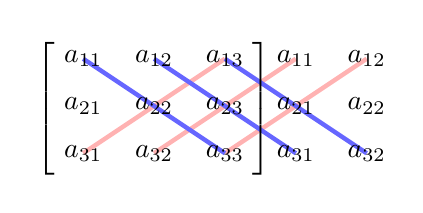
\begin{tikzpicture}[yscale=0.6,xscale=0.9]
    \draw[ultra thick,red!30] (1,-3) -- (3,-1);
    \draw[ultra thick,red!30] (2,-3) -- (4,-1);
    \draw[ultra thick,red!30] (3,-3) -- (5,-1);
    \draw[ultra thick,blue!60] (1,-1) -- (3,-3);
    \draw[ultra thick,blue!60] (2,-1) -- (4,-3);
    \draw[ultra thick,blue!60] (3,-1) -- (5,-3);
    \foreach\i in {1,2,3} {
      \foreach\j in {1,2,3} {
        \path (\j,-\i) node {$a_{\i\j}$};
      }
    }
    \foreach\i in {1,2,3} {
      \foreach\j in {1,2} {
        \path (\j,-\i) + (3,0) node {$a_{\i\j}$};
      }
    }
    \draw(0.5,-2) node {$\left[\rule{0mm}{1.0cm}\right.$};
    \draw(3.5,-2) node {$\left.\rule{0mm}{1.0cm}\right]$};
  \end{tikzpicture}
\end{equation*}
Here, we have written down the matrix $A$, then repeated the first two
columns next to it. The blue lines correspond to the positive terms of
the determinant: $\color{blue}a_{11}a_{22}a_{33}$,
$\color{blue}a_{11}a_{22}a_{33}$, and
$\color{blue}a_{13}a_{21}a_{32}$. The pink lines correspond to the
negative terms: $\color{red}a_{31}a_{22}a_{13}$,
$\color{red}a_{32}a_{23}a_{11}$, and $\color{red}a_{33}a_{21}a_{12}$.

\begin{example}{A $3\times 3$ determinant}{3-by-3-determinant}
  Find $\det(A)$, where
  \begin{equation*}
    A = \begin{mymatrix}{rrr}
      0 & 1 & 2 \\
      3 & 1 & 0 \\
      1 & 1 & -1 \\
    \end{mymatrix}.
  \end{equation*}
\end{example}

\begin{solution}
  We have
  \begin{equation*}
    \det(A) ~=~
    \begin{absmatrix}{rrr}
      0 & 1 & 2 \\
      3 & 1 & 0 \\
      1 & 1 & -1 \\
    \end{absmatrix}
    ~=~
    0\cdot 1\cdot (-1)
    + 1\cdot 0 \cdot 1
    + 2 \cdot 3 \cdot 1
    - 1\cdot 1\cdot 2
    - 1\cdot 0\cdot 0
    - (-1)\cdot 3\cdot 1
    ~=~ 7.
  \end{equation*}
\end{solution}
